\chapter{Literature Review}
\label{lit_review} % For referencing the chapter elsewhere, use \ref{intro} 
This chapter provides a review of all related works in the field of recommender systems. The chapter first focuses on the background and origin of recommender systems and outlines their main applications. This is then followed by an overview of the methods used to evaluated the accuracy and effectiveness of recommender systems. Then, the two main categories of approaches to recommender systems are discussed, namely \textit{content-based} and \textit{collaborative filtering} systems. Finally, the chapter is concluded by evaluating the top submissions to the Netflix Prize, a contest that was held in 2008, which was a major event in the progression of collaborative filtering algorithms.

\section{Introduction to Recommender Systems}
As the world has become more digitally connected, people too have become connected to an increasing number of options. When trying to decide on what movie to watch, or what album to listen to, people are presented with a vast number of options that can, oftentimes, be overwhelming. To help people in making decisions such as these, inspiration is often taken from friends' word of mouth, reviews from critics, or general surveys. Recommender systems provide an automated means for helping people discover new items \parencite{rs_1.1_Resnick}.

The goal of a recommender system can be defined as predicting the response of a user for new items, based on historical information, and suggesting novel and/or original items for which the estimated response is positive \parencite{handbook_1.4_neighbourhood}.

\subsection*{Approaches to Recommender Systems}
Recommender systems can be divided into two broad categories. \textbf{Content-based} recommender systems make use of meta data for generating recommendations. Examples of item meta data include the genre of a musical artist or song, or the director of a movie. For users, meta data such as demographic information might be used. This meta data is used to match users to items based on matching tags - the recommendations for a user who likes work of a certain author, for example, might include other books by the same author or books of the same genre \parencite{di2012linked}.

There have been a number of successful content-based recommender systems. Many web recommenders use a keyword-based technique to match web pages based on the frequency of words on the page. In movie and book recommenders, a common approach is to use similarities between the text descriptions to match products. \parencite{handbook_1.3_content-based}

One major obstacle to content-based approaches is the lack of sufficient meta data, which can be time-consuming and costly to collect. \parencite{cf_1.6_implicit}

An alternative approach, known as \textbf{collaborative filtering} (CF), uses only the historical interaction behaviour between users and items to make recommendations \parencite{cf_1.1}. This is the approach that will be investigated in this project and will be described in more detail below.

\section{Evaluating Recommender Systems}
Before expanding on the intricacies of collaborative filtering, it is first necessary to discuss the methods and metrics that are commonly used to evaluate recommender systems. This is the most subjective aspect of the process, since the success of the system depends on the objectives of its designer. For example, the intent could be to stretch customer spend, or it could be to encourage users to discover new products. In each of these cases, success would be measured using different yard sticks \parencite{eval_colab}.

There are three main approaches for evaluating the success of a recommender system. The first approach is to evaluate the system offline, without any form of user testing. The other two approaches involve user testing; either using small groups of subject matter experts, or a more large-scale approach using online user testing. While each recommender system can be evaluated subjectively based on its ability to meet certain outcomes, there are certain measurable properties which can be used to compare different systems \parencite{handbook_1.8_evaluation}. The intended outcomes of the recommender system will determine whether it can be evaluated offline, or if it will require expert or user group online testing.

\subsection{Offline Evaluation}
Most recommender systems are scored and assessed on their ability to predict known user ratings. In this case, the models have been trained to predict the numeric values of ratings that users will assign to items. The predicted values can be compared to the true ratings using common regression metrics such as mean absolute error (MAE) or root mean square error (RMSE) \parencite{eval_coverage}. If we use $P$ and $O$ to denote the ordered sets of predicted and observed user ratings respectively, and $n$ to represent the total number of user-item interactions, then the accuracy of the recommender system can be measured as

\begin{equation}
    \text{MAE} = \dfrac{|P - O|}{n}
\end{equation}
or
\begin{equation}
    \text{RMSE} = \sqrt{\dfrac{(P - O)^{2}}{n}}.
\end{equation}

However, there are alternative metrics that aim to better reflect the quality perceived by users of the system \parencite{eval_colab}.

Prediction \textbf{coverage} provides a measure of how well the recommender system is able to encourage users to explore all of the item space. If $I$ is used to denote all items available to users and $I_p$ to denote all items recommended by the recommender system, then coverage can be measured as

\begin{equation} \label{eqn:cov}
    \text{coverage} = \dfrac{|I_p|}{|I|},
\end{equation}
which is the total number of items recommended by the system divided by the total number of items contained in the training data \parencite{eval_coverage}.

In some cases, a recommender system could achieve high levels of both accuracy and coverage, but still struggle to recommend new items to users. \cite{eval_colab} used the example of a recommender system that suggests bananas to shoppers in a grocery store: \textit{"Statistically, this recommendation is highly accurate: almost everyone buys bananas. However, everyone who comes to a grocery store to shop has bought bananas in the past, and knows whether or not they want to purchase more. Further, grocery store managers already know that bananas are popular, and have already organised their store so people cannot avoid going past the bananas."} 

It should be noted, however, that a recommender system should not \textit{only} recommend unexpected items. As \cite{swearingen2001beyondalgorithms} showed, non-novel recommendations help to develop trust from users in the system and should be combined with more unexpected suggestions to provide an enjoyable overall user experience.

\textbf{Serendipity} is a metric that has been used to assess both a recommendation's unexpectedness \textbf{and} its usefulness \parencite{online_predicting}. Serendipity is more of a conceptual evaluative measure, rather than a fixed formula like RMSE. One approach to capture serendipity numerically has been suggested by \parencite{eval_colab}. In the case where a recommender can produce expected probabilities for a given user for every item in the system, fir example, one could divide each probability by the average user probability score to produce re-weighted scores. The resulting probabilities would represent a measure of how much more likely a given user is to like items than the average user.

In the case where ratings are not available -- that is when only a list of user-item interactions is given -- the task of providing recommendations is often transformed into one of providing a set number of items to a user. Using $P$ to denote the set of items that are suggested to the user and $O$ to denote the set of items which the user was observed to have preferred, this type of approach can then be evaluated using \textbf{precision} and \textbf{recall}, computed as

\begin{equation}
    \text{precision} = \dfrac{|P \cup O|}{|P|}
\end{equation}
and
\begin{equation}
    \text{recall} = \dfrac{|P \cup O|}{|O|}
\end{equation}
\parencite{handbook_1.4_neighbourhood}.

\subsection{Online Testing}
Testing recommender systems in an online manner, be it user studies or large-scale trials, requires a large enough audience that can be split into test and control groups. Ideally, the two user groups would be identical apart from the fact that the test group would receive suggestions from the recommender system, while the control group would not. The two groups would then be assessed on their behaviour over a trial period, allowing for the recommender system to be assessed in various areas such as uplift in incremental sales or exploration of the item space \parencite{online_predicting}.

An example of online testing can be found in the work done by \cite{swearingen2001beyondalgorithms}, where users were asked to evaluate a number of internet recommender systems and compare their suggestions to those of their friends. Users were asked to classify which recommendations they received were good, and then to further distinguish between \textbf{useful} recommendations they had never seen before and \textbf{previously liked} recommendations. One particularly interesting observation from this study was that recommender systems tended to produce more suggestions of completely new items than friends, who tended to recommend items of which users were already aware.

The advantage of testing recommender systems in this way is that it affords the systems the chance to influence a user's interaction behaviour. Indeed, recommender systems exist for the main purpose of suggesting items to users that they are predicted to like, but would otherwise not have known about. The influence of a recommender system cannot be assessed through back-testing. It can only be done through online trials \parencite{handbook_1.4_neighbourhood}.

Since each system needs its own independent test group, the size of the audience required only increases with the number of recommender systems being compared, which makes online testing infeasible in the context of this master's dissertation. Therefore, all comparisons between recommender systems in this paper will be made using offline metrics.

\subsection{Netflix Prize}
A major event in the progression of recommender system methods, as well as the evaluative metrics thereof, was the 2006 Netflix Prize. In 2019, Netflix is a well-known online video subscription service that provides content to subscribers through streaming. However, in 2006 Netflix was an online video subscription service that provided DVD rentals to subscribers via the mail. As part of their service, they encouraged users to rate movies that they watched which resulted in the creation of a data set of some 1.9 billion ratings from 11.7 million subscribers across 85 thousand titles in under 10 years \parencite{netflix_description}.

This data set was used by Netflix to create their own recommendation algorithm, which was known as Cinematch. Cinematch used a variant of Pearson's correlation to determine a movie's similarity to all other movies. These similarities between movies were used to provide personalised recommendations to users based on the movies they had rated. The main method used to assess the performance of Cinematch was to compute the RMSE between the predicted and observed user ratings \parencite{netflix_description}.

In 2006, Netflix released a variation of this data set to the data science community at large with the challenge of improving on the performance achieved by the existing Cinematch algorithm. The data set provided for this challenge contained over 100 million ratings (and their dates) from over 480 thousand subscribers on almost 18 thousand movies. The data were collected between 1998 and 2005, and comprised a representative sample of all ratings captured by Netflix during this period. The user ratings were measured on an integer scale from 1 to 5. Three million of the most recent ratings from those same subscribers across the same set of movies was withheld as a competition qualifying set. Half of the qualifying data set was used to compute the RMSE of submissions onto the running public leader board, while the other half, known as the "quiz" subset was used by Netflix to decide the eventual winning team \parencite{netflix_description}.

As a reference for competition contestants, Netflix reported that the Cinematch algorithm was able to achieve a performance of 0.9514 RMSE on the quiz subset, which was 9.6\% lower than simply predicting using the average movie ratings \parencite{netflix_description}.

Figure \ref{fig:netflix_submissions} shows the relative distribution of the submissions' performance with respect to that of the Cinematch algorithm. The figure was created in 2007, at which point no team had achieved the goal of a 10\% improvement over Cinematch. The numbers in red correspond to submissions in which the same value is used for every prediction, while the "wooden spoon" was the lowest score achieved by any of the entrants. Interestingly, a significant number of submissions achieved RMSE scores lower than would be achieved by predicting every rating to be 4.

\begin{figure}[H]
\centering
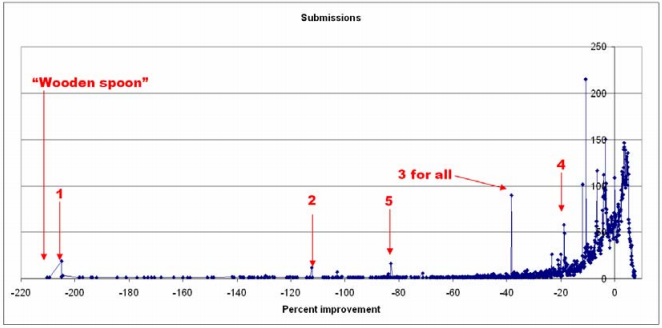
\includegraphics[width=13cm]{Figures/2_1_netflix-prize.png}
\decoRule
\caption[Netflix submissions]{Netflix prize submissions ordered by improvement over Cinematch \parencite{netflix_description}.}
\label{fig:netflix_submissions}
\end{figure}

However, in 2008, the competition reached its conclusion, when the team known as "BellKor's Pragmatic Chaos" surpassed the 10\% improvement level \parencite{netflix_bellkor}.

\section{Collaborative Filtering}
The term ``collaborative filtering'' was first coined by \cite{cf_1.3_origin}, who used it to refer to a system for suggesting relevant emails for a person from a selection of mailing lists. This system incorporated the reactions of other users in the filtering process.

Since then, the term has generally been used to describe a process through which known preferences of users in a group are used to predict the unknown preferences of other users \parencite{cf_1.1}. In most cases, the preferences of users within the group are indicated by a rating or score of some kind; for example, users might assign positive ratings to items they liked, and negative ratings to items they did not. The term \textit{collaborative} refers to the fact that the users of the system improve its performance with each rating that they contribute \parencite{cf_1.2_eigentaste}, i.e., as users record more ratings of items, the ability of the system to \textit{filter} accurate recommendations for other users improves. 

Collaborative filtering techniques provide an algorithmic method for making recommendations to users, based on the preferences of other similar users. The fundamental assumption that underlies CF techniques is that users who have rated $k$ items similarly will also rate other items similarly. For example, if user $A$ likes movies $m_1$, $m_2$, $m_3$, and user $B$ likes movies $m_1$, $m_2$, $m_3$, $m_4$, then user $A$ is also likely to enjoy movie $m_4$ \parencite{cf_1.1}.

One of the advantages of collaborative filtering is that it can be performed without any meta data relating to either the users or the items in the database. Whereas other predictive models make predictions for a response variable using the values of one or more predictor variables, CF models make predictions for ratings using only other ratings \parencite{handbook_1.1_intro}.

One issue with content-based approaches is their limited capacity to recommend novel, unexpected items. The system will recommend items which match highly to a user's known preferences, i.e. they are limited by the user's tendency for exploration. \parencite{handbook_1.3_content-based}

Collaborative-filtering-based models, on the other hand, leverage the collective experiences of all users to recommend interesting new items to users. In contrast to content-based models, models that employ collaborative filtering are known to produce serendipitous recommendations that users would not typically expect \parencite{herlocker2002empirical}.

\subsection{User Feedback}
 In collaborative filtering recommender systems, the inputs are provided by people (users) who rate items with which they have interacted \parencite{cf_1.5_explicit}. The function of a recommender system is to aggregate these ratings from users to make recommendations to other users on which items they might like. In some cases, ratings are provided to a recommender system explicitly by users, but in many other cases these ratings have to be inferred based on user-item interactions \parencite{cf_1.6_implicit}. 

\subsubsection{Explicit Ratings}
Explicit feedback is captured when a user makes the conscious decision to \textit{explicitly} rate an item. These ratings can be binary (e.g.\ like or dislike), numeric (e.g.\ 1-10 rating scale) or unstructured (e.g.\ annotated text). For example, a user can indicate that they like a certain song by giving it a "thumbs up" on a music streaming service \parencite{cf_1.5_explicit}.

This type of feedback directly captures user preferences towards items; however, it can be scarce. It has also been found that the rate at which users provide explicit feedback decreases over time and, furthermore, that leaving feedback has a negative effect on user behaviour overall \parencite{cf_1.5_explicit}. This is shown in figure \ref{fig:playcount} where the average percentage of loved tracks over all users is shown to decrease as playcount increases.

\begin{figure}[H]
\centering
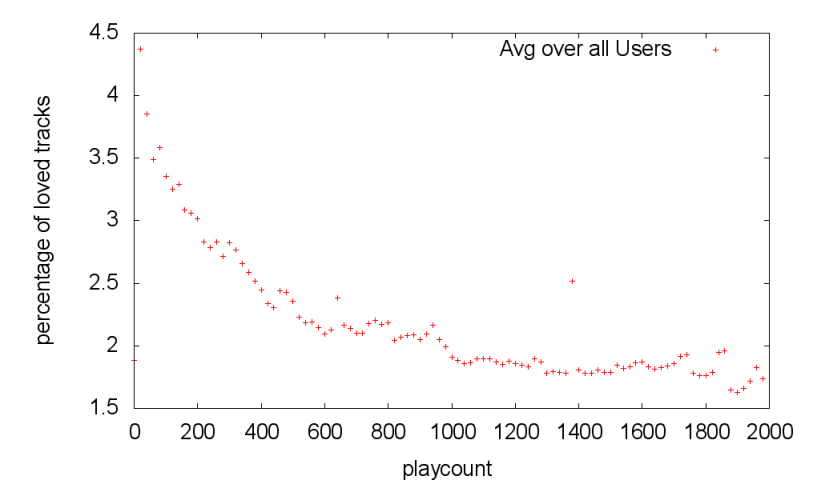
\includegraphics[width=13cm]{Figures/2_2_playcount-vs-loved.png}
\decoRule
\caption[Playcount-loved]{Percentage of loved tracks as playcount increases \parencite{cf_1.5_explicit}.}
\label{fig:playcount}
\end{figure}

\subsubsection{Implicit Feedback}
Alternatively, the user might not explicitly rate items they like, in which case a recommender system would need to infer their preferences from their interaction history. Using the example of a music streaming service, many users do not choose to 'like' or rate songs; however, they will tend to listen to songs they like more often than those they do not. \cite{cf_1.5_explicit}, showed that there is a positive correlation between the number of 'likes' a track receives from users and its total play count. Therefore, it is a viable option to infer positive feedback from user interaction data. Other forms of implicit feedback include purchase history, browsing and search patterns, or mouse movements and click patterns \parencite{handbook_1.5_cf}.

Whether the user feedback is implicit or explicit, the job of the recommender system is the same - to aggregate this feedback from users to aid others in discovering new items of interest. It has been shown that using a combination of explicit and implicit feedback can yield improved recommendation accuracy \parencite{cf_1.4_comparison}; however, it is the subtleties around \textit{how} recommender systems identify all the signals from the available user feedback data that remains the greatest area of focus for improving accuracies.

\subsection{Neighbourhood-based Recommender Models}
There are two main techniques used in collaborative filtering recommender systems: \textit{neighbourhood-based} and \textit{latent factor} models \parencite{handbook_1.5_cf}. As the name suggests, neighbourhood models employ a nearest-neighbours approach to recommending items to users.

Neighbourhood-based approaches were some of the most prevalent in the early years of recommender systems at the end of the 90s. These methods make use of similarity measures to select subsets -- or neighbourhoods -- of users or items \parencite{cf_1.6_implicit}. These neighbourhoods are used to produce weighted average ratings to generate predictions for users \parencite{herlocker1999algorithmic}.

\subsubsection{User-based similarity}
The first types of neighbourhood models estimated unknown ratings using a user-oriented approach in which predictions were based on the known ratings of like-minded users \parencite{cf_1.6_implicit}.

To make a prediction for a given user $a$ for item $i$, the first step is to measure their similarities to all other users of the system. Similarity between users $a$ and $u$ can be calculated using the Pearson correlation coefficient, $w_{a,u}$, computed as
\begin{equation}
    w_{a,u} = \dfrac{\sum\limits_{i=1}^{m}[(r_{a,i}-\bar{r}_a)(r_{u,i}-\bar{r}_u)]}{\sqrt{\sum\limits_{i=1}^{m}(r_{a,i}-\bar{r}_a)^2\sum\limits_{i=1}^{m}(r_{u,i}-\bar{r}_u)^2}},
\end{equation}
where $r_{a,i}$ is the rating for the active user $a$ of item $i$ and $\bar{r}_a$ is their average rating, while $m$ is the set of items covered by either user.

This similarity can then be used to predict the rating for the active user for item $i$ as
\begin{equation}
    P_{a,i} = \bar{r}_a + \dfrac{\sum\limits_{u \in N(a)}w_{a,u}(r_{u,i}-\bar{r}_u)}{\sum\limits_{u \in N(a)}w_{a,u}},
\end{equation}
where $N(a)$ is the set of user $a$'s neighbours \parencite{herlocker2002empirical}.

This approach was modified by \cite{shardanand1995social}, who used a constrained Pearson correlation coefficient, calculated as
\begin{equation}
    w_{a,u} = \dfrac{\sum\limits_{i=1}^{m}[(r_{a,i}-4)(r_{u,i}-4)]}{\sqrt{\sum\limits_{i=1}^{m}(r_{a,i}-4)^2\sum\limits_{i=1}^{m}(r_{u,i}-4)^2}}.
\end{equation}
The value 4 was used as it was the midpoint of the seven-point rating scale on which their music recommendation system, dubbed "The Ringo", was based. The number of neighbours was limited by applying a correlation threshold, where only users above the threshold could be considered for membership to the neighbourhood. Increasing the magnitude of this threshold resulted in greater accuracy, but limits the number of items for which the system can make recommendations \parencite{herlocker2002empirical}.

The most common alternative similarity measure to the Pearson correlation coefficient is the cosine similarity, which is calculated between users $a$ and $u$ as
\begin{equation}
    \cos(r_a,r_u) = \dfrac{(r_a\cdot r_u)}{||r_a||\times||r_u||},
\end{equation}
where $a$ and $u$ represent the ratings vectors for each user, considering only items which have been rated by both users, $r_a\cdot r_u$ is the dot product of the two rating vectors and $||r_a||\times||r_u||$ is the product of their magnitudes \parencite{handbook_ch2}.

This measure can then be used to make a prediction for user $a$ and item $i$ by selecting the $n$ most similar neighbours and taking an average of their rating of the item, weighted by their cosine similarity.

Though the Pearson correlation and cosine similarity are the most popular measures used, it is possible to use any other common distance measure, such as the Euclidean or Minkowski distance \parencite{handbook_ch2}.

\subsubsection{Item-based similarity}
An alternative to neighbourhood models is an item-oriented approach, in which the known ratings of a user for similar items are used to make a prediction for a new item \parencite{cf_1.6_implicit}. When making a prediction for user $a$ and item $i$, all known ratings of the user are used as the neighbourhood. The predicted rating is taken as the average of all known ratings, weighted by their corresponding item similarity with $i$. The similarity measure for this neighbourhood can be any of the same measures as used in the user-based approach, only in this case the similarities are measured between items instead of users \parencite{handbook_1.4_neighbourhood}.

\subsection{Latent Factor Recommender Models}
Latent factor models attempt to characterise both users and items using anywhere in the region of between 20 to 100 factors. These latent factors capture behavioural patterns between users and items in the ratings space \parencite{koren2009matrix}.

The most common version of latent factor model is the matrix factorisation (MF) method, used by \cite{bellkor_2008} to win the Netflix Prize. In this approach, the user/item interaction data is represented as a matrix which is then factorised as the product of two lower rank matrices. 

Figure \ref{fig:2_matrix-decomposition} shows the matrix representation of the explicit interactions between users and items. All blue values are known ratings submitted by users, while the white zeroes represent unknown values which need to be predicted. Each row thus holds the ratings made by a particular user and each column the ratings received by a single item. The rating made by user $i$ of item $j$ can be found in the $j^{th}$ column of row $i$.

\begin{figure}[H]
\centering
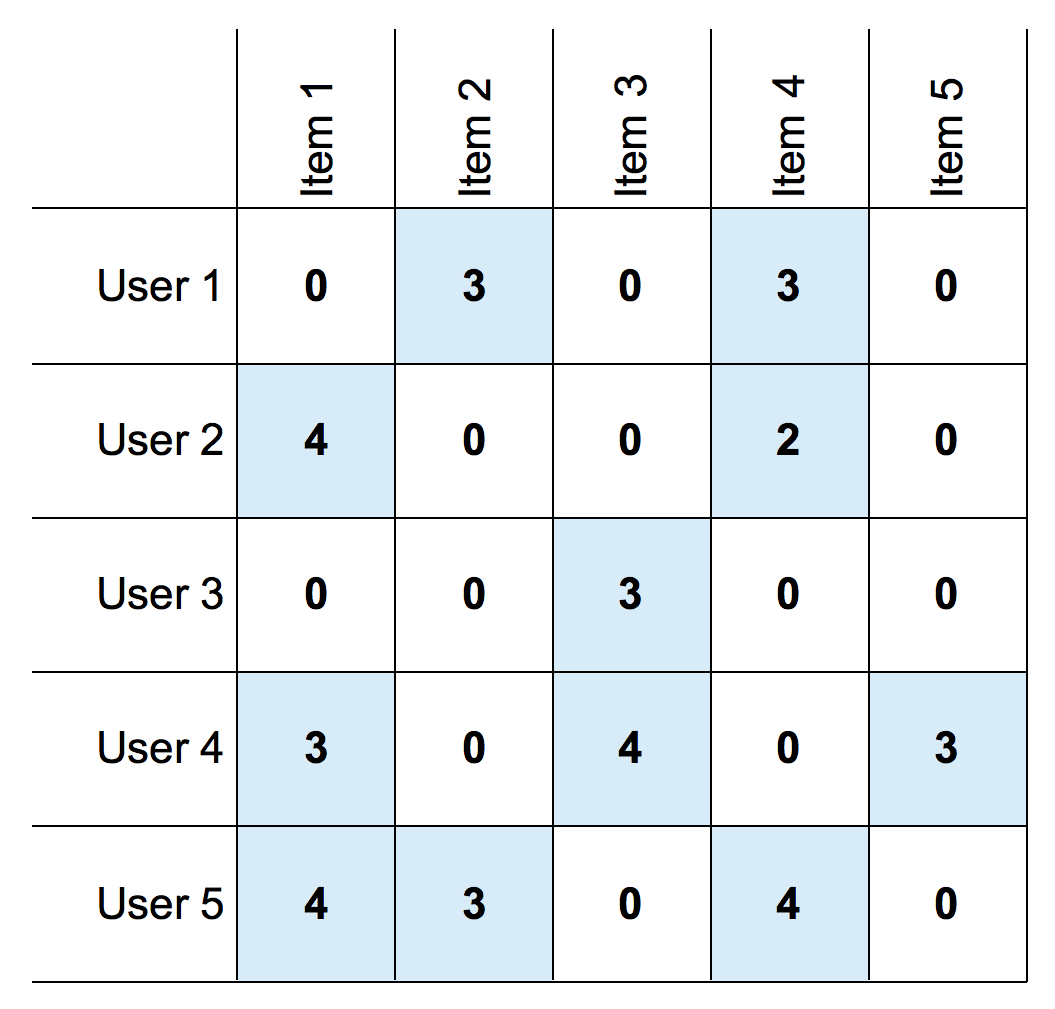
\includegraphics[width=6cm]{Figures/2_3_matrix.png}
\decoRule
\caption[Ratings matrix]{Interactions between users and items represented as a matrix \parencite{bailey_2016}.}
\label{fig:2_matrix-decomposition}
\end{figure}

If the ratings matrix consists of $m$ rows and $n$ columns, then any two matrices of dimensions $m$ x $d$ and $n$ x $d$ respectively, when cross multiplied together, would result in a matrix of the same dimensions as the original ratings matrix. The common dimension, $d$, is a hyperparameter which represents the number of latent factors, where $d <= \min(m,n)$ \parencite{bailey_2016}.

\begin{figure}[H]
\centering
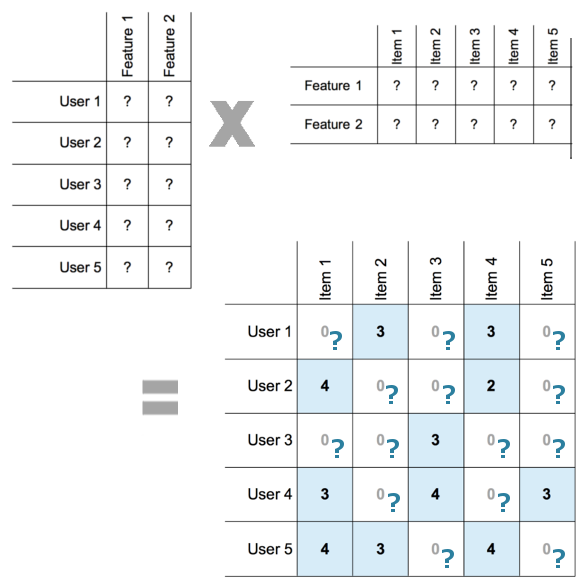
\includegraphics[width=9.5cm]{Figures/2_4_matrix_factorization.png}
\decoRule
\caption[Matrix decomposition]{Ratings matrix factorised as product of two latent factor matrices \parencite{bailey_2016}.}
\label{fig:factors}
\end{figure}

To get the rating for the first user of the first movie, one takes the dot product of the first row of the user matrix with the first column of the item matrix. More generally, the rating made by user $i$ of item $j$ is calculated as

\begin{equation}
    \hat{r}_{ij} = p_i \cdot q_j^T,
\label{eqn:dot_prod}
\end{equation}

where $p_i$ is the $i^{th}$ row of the user latent factor matrix and $q_j$ is the $j^{th}$ column of the item latent factor matrix.

\subsubsection{Optimisation techniques}
The two latent factor matrices that are used in the MF approach need to be \textit{learnt}. Their values can be solved through either stochastic gradient descent or alternating least squares (ALS), optimising the minimal distance between the original ratings matrix and the reconstructed matrix. The ALS optimisation technique was the favoured approach taken by \cite{bellkor_2008}. This technique holds the values in one factor matrix fixed and then uses least squares to solve the values in the other and \textit{vice versa}. The converged solution provides the closest reconstruction of the original ratings matrix, with the missing values filled in \parencite{koren2009matrix}.

The two resulting latent factor matrices consist of vectors which describe both the users and the items respectively. For each user and item, there will be $d$ latent factors which represent their characteristics. In the case that the items are movies, the latent factors might represent known dimensions, like genres such as comedy or romance. They might also represent deeper dimensions, like dialogue style or the amount of satire. The latent factors might also represent completely uninterpretable dimensions too. In the case of users, the latent factors represent their partiality to the corresponding item latent factor \parencite{koren2009matrix}.

\subsubsection{Biases}
The MF approach may be extended to include biases which compensate for systematic tendencies across both users and items. For example, some users tend to rate all items higher or lower than average, and some items might be generally over-rated by all users \parencite{koren2009matrix}.

When incorporating biases, equation \ref{eqn:dot_prod} becomes
\begin{equation}
    \hat{r}_{ij} = \mu + b_i + b_j + p_i \cdot q_j^T,
\label{eqn:dot_bias}
\end{equation}
where $\mu$ is the overall average rating and $b_i$ and $b_j$ are the biases of user $i$ and item $j$.

\subsubsection{Netflix Prize winning submission}
The winning submission to the Netflix Prize made use of an ensemble model, achieving an RMSE of 0.8712 on the test set using a combined total of over 500 models which included MF, restricted Boltzmann machines and nearest neighbour models. Despite this extensive range of models used in their winning ensemble, the team members noted that the most accurate standalone approach was to use MF \parencite{netflix_bellkor}. 

Aside from the choice of algorithm(s), the winning team paid special attention to what they termed "baseline predictors". The purpose of these was to "encapsulate those effects which do not involve user-item interaction." This method meant that predicted ratings were decomposed into multiple parts and is not dissimilar to how equation \ref{eqn:dot_bias} represents predicted ratings. In this equation, the first three terms can be considered baseline features, while the final term, $q_i^T p_u$, represents the specific user-item interaction. For example when predicting how a user, Alice, might rate the movie Inception, the prediction would first consider the average rating of the movie, as well as the average of all of Alice's ratings as the baseline predictors. Then, the specific user-item interaction is made using the latent features and is used to adjust the baseline prediction. In addition to user and item biases, temporal aspects were used to adjust the baseline. Factors such as time since a user's first rating and how many ratings a user made on a particular day were found to have a significant impact on user ratings. To capture temporal effects, the user and item biases were each calculated as a function of time. 

When accounting for temporal components, equation \ref{eqn:dot_bias} becomes

\begin{equation}
    \hat{r}_{ui} = \mu + b_u(t_{ui}) + b_i(t_{ui}) + q_i^T p_u,
\label{eqn:temp_baseline}
\end{equation}

where $b_u$ and $b_i$ are functions that change over time \parencite{netflix_bellkor}.

\subsection{Uses of deep learning in collaborative filtering}
Tremendous effort was required from all of the contestants of the Netflix Prize competition to push the boundaries of predictive ability in CF models. Ensemble models and intricate modelling of baseline predictors were used to eek out marginally better models; however, it was shown that the improvement in accuracy was largely due to the use of latent factors. Then, it was through the use of matrix decomposition that these latent factors were learnt; however neural networks can perform the same task through the use of embedding layers, with the added ability of learning non-linear patterns in the data.

The first notable use of deep learning for collaborative filtering was in \cite*{sedhain2015autorec}, when \citeauthor{sedhain2015autorec} used an autoencoder framework for their \textit{AutoRec} model. They opted for an item-based approach in which the input to the neural network is a partially observed vector containing all user ratings for a given item. Figure \ref{fig:autorec-arch} shows the architecture of this model.

\begin{figure}[H]
\centering
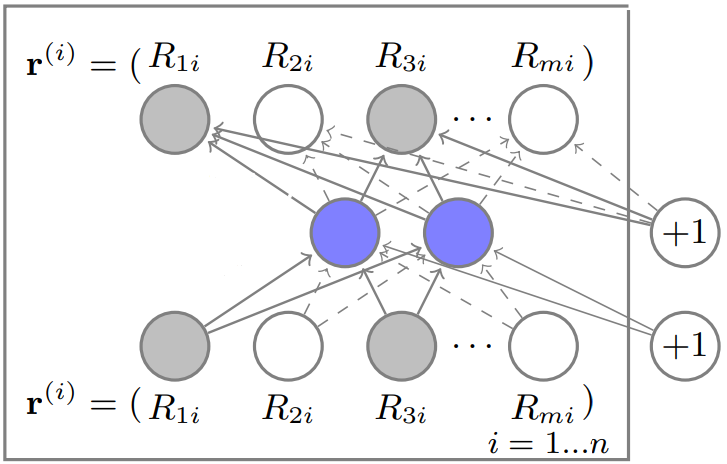
\includegraphics[width=8cm]{Figures/2_autoRec.png}
\decoRule
\caption[AutoRec]{AutoRecu uses an autoencoder architecture  \parencite{sedhain2015autorec}}
\label{fig:autorec-arch}
\end{figure}

It can be seen in figure \ref{fig:autorec-arch} that the input dimension of the AutoRec model is equal to the number of users, $m$. There are $n$ copies of the network, one for each item. Since each input is sparse, only the parameters associated with the observed ratings are updated during backpropagation. This means that the trained model takes as input a sparse item ratings vector, representing all available user ratings for that item, and outputs a complete ratings vector containing all predicted user ratings for the item \parencite{sedhain2015autorec}.

Evaluation of this model was done using the MovieLens 1M, 10M and Netflix datasets using 5 separate random 90\%-10\% train-test splits, with 10\% of the training data being used for hyperparameter tuning. Test accuracy was taken as the average of these 5 random splits and users or items in the test set without training observations were given a default rating of 3 stars. They reported test accuracies of 0.831, 0.782 and 0.823 on the MovieLens 1M, 10M and Netflix datasets respectively \parencite{sedhain2015autorec}.

Figure \ref{fig:autorec-arch} shows the item-based AutoRec model.
\citeauthor{sedhain2015autorec} experimented with a user-based model, taking $n$-dimensional user rating vectors as inputs to $m$ copies of the network. However, they found this model achieved reduced accuracy, likely due to the fact that there are more items per movie than per user in the datasets they used.

A neural architecture was used in the "Neural Collaborative Filtering" (NCF) model created by \cite{he2017neural}. This particular effort focused on the CF scenario where only implicit feedback is used; however, the architecture used is equally suited to using explicit feedback. Figure \ref{fig:ncf-arch} shows the architecture of a NCF model, with $X$ hidden units and $k$ latent factors.

\begin{figure}[H]
\centering
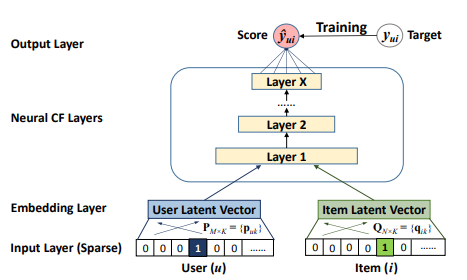
\includegraphics[width=9.5cm]{Figures/2_neural-cf.png}
\decoRule
\caption[Neural Collaborative Filtering]{Neural Collaborative Filtering architecture \parencite{he2017neural}}
\label{fig:ncf-arch}
\end{figure}

The NCF model generalises MF through the use of an embedding layer, which combines both user and item latent factors. The embedding layer serves the same purpose as the latent factor matrices in the MF approach, while the hidden layers allow for non-linear combinations of these latent factors when predicting ratings.

Although the results achieved by \citeauthor{sedhain2015autorec} represented an improvement of more than 5\% on the winning submission to the Netflix Prize, it should be noted that their method of evaluation on the Netflix set was not equivalent to the true holdout set used in the competition.

Finally: \parencite{rendle2019difficulty} and \parencite{dacrema2019we}.

\section{Transfer learning}
The literature that has been reviewed in the previous sections of this chapter has covered the topic of recommender systems, with specific focus on tasks related to predicting explicit ratings using CF. While questions have been raised regarding the reproducibility of some results that claim to have improved on the state of the art, \parencite{dacrema2019we}, there can be no questioning the effectiveness of latent factor models for learning otherwise-unknown features of the user and item sets.

The aim of this masters dissertation is to predict genre labels of items, such as movies or books, that have been rated explicitly by users. The prediction of genres requires latent features to be learnt through the task of predicting ratings. These latent features can then be re-used in a second model to predict genres. This process is named collaborative genre tagging (CGT) This process of adapting the learnings of one model in order to train another places CGT under the domain of transfer learning.

\cite{ruder2019state} describes transfer learning as \textit{"a means to extract knowledge from a source setting and apply it to a different target setting"}. Its use has allowed for image classifiers to be created by fine tuning convolutional neural networks, achieving state-of-the-art performance in a wide variety of computer vision tasks while using significantly less data for training \parencite{sharif2014cnn}. Any machine learning scenario in which knowledge is gained from one task and re-used for another is considered transfer learning, as can be seen in figure \ref{fig:transfer-scenario}.

\begin{figure}[H]
\centering
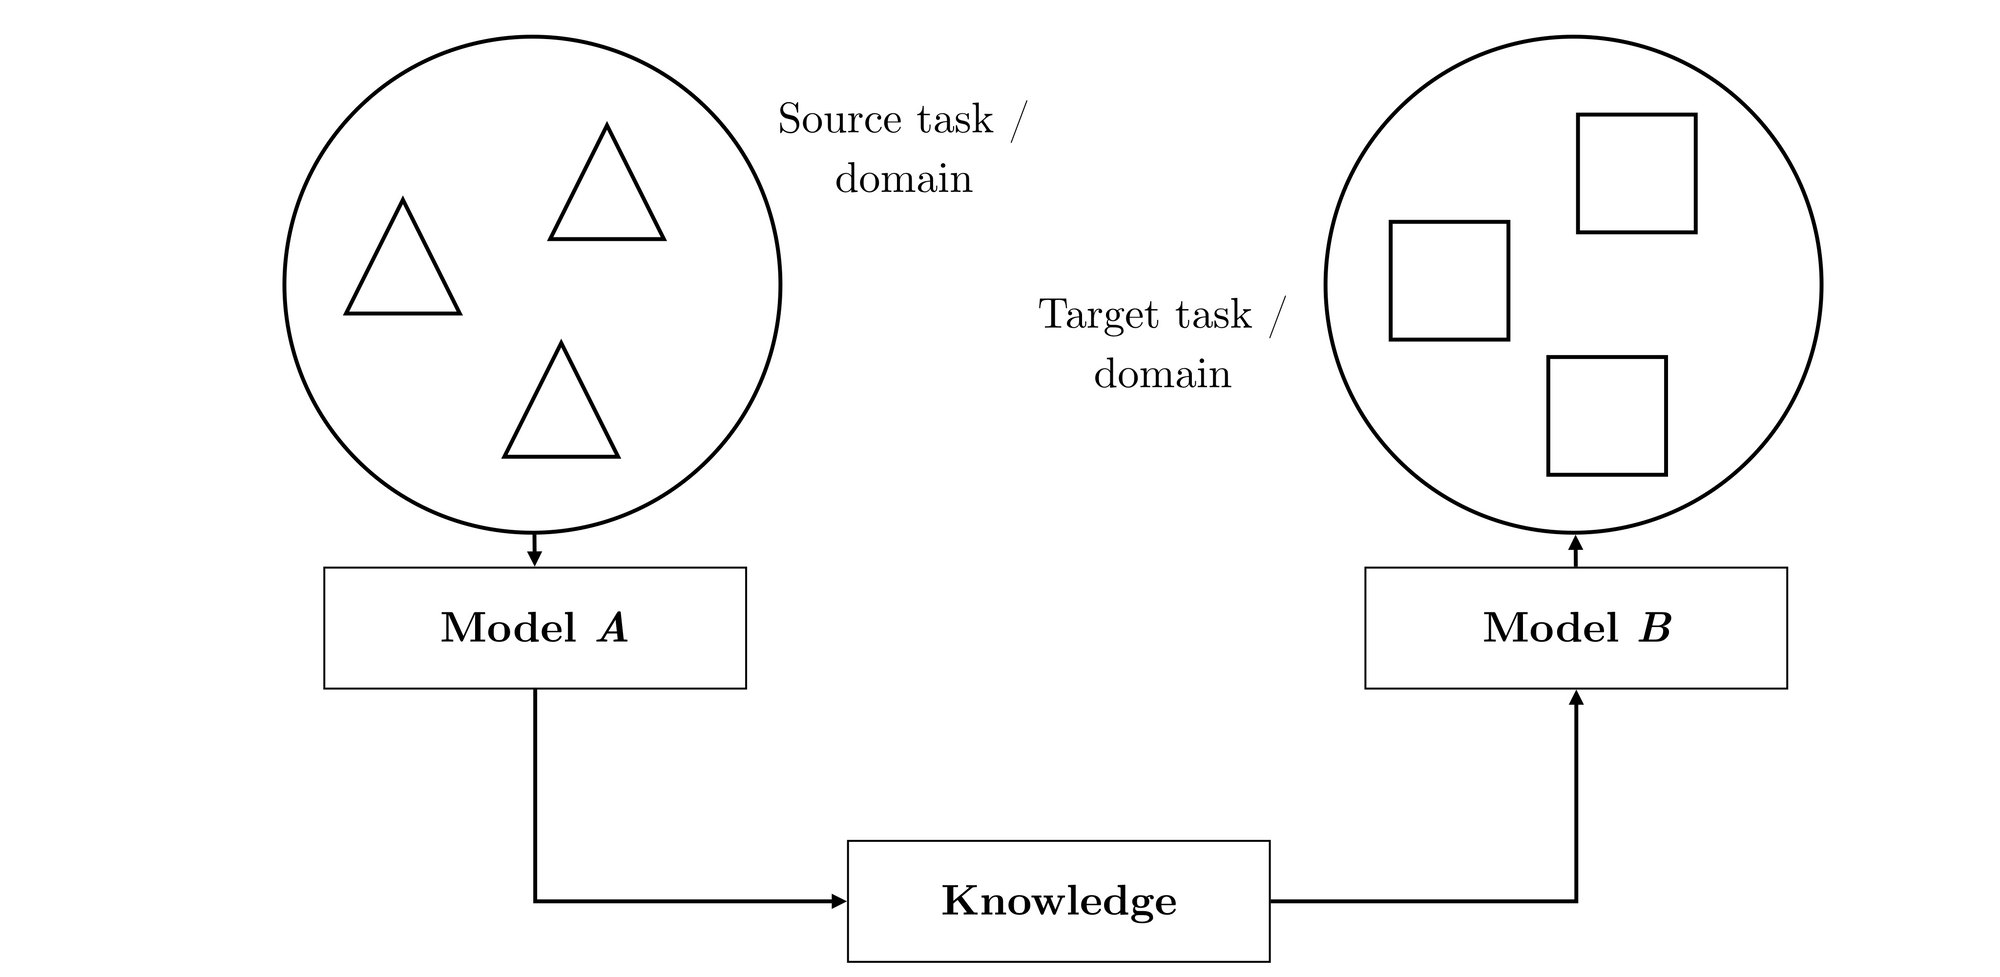
\includegraphics[width=0.8\textwidth]{Figures/2_transfer-learning-scenario.png}
\decoRule
\caption[Transfer Learning Scenario]{The transfer learning scenario \parencite{ruder2019state}}
\label{fig:transfer-scenario}
\end{figure}

\cite{collobert2011natural} demonstrated the effectiveness of using word embeddings for a variety of natural language processing tasks. Word embeddings can be learned through trainable layers in a neural network that extract a set of features for each word. For each word, a set of features is stored in a lookup table. These features can be trained using unlabelled datasets, such as the entire corpus of the English Wikipedia. By removing words from sentences in the corpus, then training a language model to predict the missing word, the word embeddings can be trained such that they capture the syntactic and semantic information associated with the words themselves. These word embeddings can then be re-used in a sequence model to perform transfer learning on tasks such as sentiment analysis or part-of-speech tagging.